%===================================================================================
% JORNADA CIENTÍFICA ESTUDIANTIL 2013 - MATCOM, UH
%===================================================================================
% Esta plantilla ha sido diseñada para ser usada en los artículos de la
% Jornada Científica Estudiantil, MatCom 2015.
%
% Por favor, siga las instrucciones de esta plantilla y rellene en las secciones
% correspondientes.
%
% NOTA: Necesitará el archivo 'jcematcom.sty' en la misma carpeta donde esté este
%       archivo para poder utilizar esta plantila.
%===================================================================================



%===================================================================================
% PREÁMBULO
%-----------------------------------------------------------------------------------
\documentclass[a4paper,10pt,twocolumn]{article}

%===================================================================================
% Paquetes
%-----------------------------------------------------------------------------------
\usepackage{amsmath}
\usepackage{amsfonts}
\usepackage{amssymb}
\usepackage{jcematcom}
\usepackage[utf8]{inputenc}
\usepackage{listings}
\usepackage[pdftex]{hyperref}
%-----------------------------------------------------------------------------------
% Configuración
%-----------------------------------------------------------------------------------
\hypersetup{colorlinks,%
	    citecolor=black,%
	    filecolor=black,%
	    linkcolor=black,%
	    urlcolor=blue}

%===================================================================================



%===================================================================================
% Presentacion
%-----------------------------------------------------------------------------------
% Título
%-----------------------------------------------------------------------------------
\title{Generación Automática de Configuraciones Visuales}

%-----------------------------------------------------------------------------------
% Autores
%-----------------------------------------------------------------------------------
\author{\\
\name Victor Manuel Cardentey Fundora 
	\\ \addr Grupo C511 \AND
\name Karla Olivera Hernández 
  \\ \addr Grupo C511 \AND
\name Amanda González Borrell 
  \\ \addr Grupo C511
  }

%-----------------------------------------------------------------------------------
% Tutores
%-----------------------------------------------------------------------------------
\tutors{\\
Lic. Daniel Alejandro Valdés Pérez \\
Lic. Ernesto Estevanell}

%-----------------------------------------------------------------------------------
% Headings
%-----------------------------------------------------------------------------------

%-----------------------------------------------------------------------------------
%===================================================================================



%===================================================================================
% DOCUMENTO
%-----------------------------------------------------------------------------------
\begin{document}

%-----------------------------------------------------------------------------------
% NO BORRAR ESTA LINEA!
%-----------------------------------------------------------------------------------
\twocolumn[
%-----------------------------------------------------------------------------------

\maketitle

%===================================================================================
% Resumen y Abstract
%-----------------------------------------------------------------------------------
\selectlanguage{spanish} % Para producir el documento en Español

%-----------------------------------------------------------------------------------
% Resumen en Español
%-----------------------------------------------------------------------------------

%-----------------------------------------------------------------------------------
% English Abstract
%-----------------------------------------------------------------------------------
% \vspace{0.5cm}

% \begin{enabstract}

%   The English Abstract must have have $100$ to $200$ words, and present in a clear
%   and concise form the essentials of the article content.

% \end{enabstract}

%-----------------------------------------------------------------------------------
% Palabras clave
%-----------------------------------------------------------------------------------
% \begin{keywords}
% 	Separadas,
% 	Por,
% 	Comas.
% \end{keywords}

%-----------------------------------------------------------------------------------
% Temas
%-----------------------------------------------------------------------------------
% \begin{topics}
% 	Tema, Subtema.
% \end{topics}


%-----------------------------------------------------------------------------------
% NO BORRAR ESTAS LINEAS!
%-----------------------------------------------------------------------------------
\vspace{0.8cm}
]
%-----------------------------------------------------------------------------------


%===================================================================================

%===================================================================================
% Introducción
%-----------------------------------------------------------------------------------
\section{Introducción}\label{sec:intro}
%-----------------------------------------------------------------------------------
 
La generación automática de visualizaciones sobre un conjunto de
    datos se puede dividir en dos procesos: determinar una consulta de interés
    para el usuario y generar la configuración gráfica para visualizar los resultados de la
    consulta. En particular la selección de configuraciones gráficas es un problema que
    presenta dificultades para llegar a consenso entre expertos del dominio y los sistemas
    tradicionales que brindan solución a este problema utilizan enfoques basados en reglas.
    En años recientes se ha planteado la posibilidad de aplicar técnicas de \textit{Machine Learning}
    ampliamente utilizadas en sistemas de recomendación tradicionales a la recomendación de configuraciones
    gráficas \cite{hu2019vizml} \cite{li2021kg4vis}. La propuesta de este trabajo consiste en utilizar y comparar distintos modelos
    de \textit{Machine Learning} en la tarea de selección de configuraciones gráficas e implementar un marco de trabajo
	para futuras investigaciones sobre el tema.

%===================================================================================



%===================================================================================
% Desarrollo
%-----------------------------------------------------------------------------------
\section{Desarrollo}\label{sec:dev}
%-----------------------------------------------------------------------------------
 
	\subsection{Definici\'on del problema}
	El proplema de elegir configuraciones gr\'aficas se define como dado un \textit{dataset} de 
	$k$ columnas elegir los valores de configuraciones gr\'aficas para visualizar estos datos, ejemplos de configuraciones gr\'aficas son el tipo de gr\'afico
	y el eje correspondiente a cada columna en dicho gr\'afico. Como convenci\'on para diferenciar el \textit{dataset} correspondiente
	a un gr\'afico del \textit{dataset} de \textit{datasets} utilizado para entrenar los modelos propuestos se utilizar\'a \textit{Plotly Dataset}
	para referirse a este u\'ltimo durante el resto de este trabajo.

	Este problema se model\'o como un problema de clasificaci\'on multiclase:
	
	Sea un conjunto $C = \{T, A\}$ de configuraciones gr\'aficas donde:
	\begin{enumerate}
		\item $T = \mathbb{N}_k$ donde $k$ es la cantidad de tipos de gr\'aficos.
		\item $A = \{a_1, a_2,...,a_k\}$ donde $k$ es la cantidad de tipos de gr\'aficos y $a_i$ es la
		cantidad de ejes v\'alidos en un gr\'afico de tipo $i$.
	\end{enumerate}
		
	Se consideraron como tipo de gr\'aficos el gr\'afico de barras, gr\'afico de l\'ineas y gr\'afico de puntos entonces $T = \mathbb{N}_3$, 
	todos estos tipos de gr\'aficos tienen dos ejes v\'alidos por lo que $\forall i \in [1,k] \; A_i = \mathbb{N}_2$.

	Se define el conjunto de posibles clases
	$$L = \{ (t_i, j): t_i \in T \;\forall j \in [1, a_i] \;\forall i \in [1,k] \}$$.

	En este caso $$L = \{ (1,1),(1,2),(2,1),(2,2),(2,1),(2,2) \}$$
	
	Estas categor\'ias pueden interpretarse como:\\
	$\{(\textbf{barra}, \textbf{eje\_x}), (\textbf{barra}, \textbf{eje\_y}),
	(\textbf{l\'inea}, \textbf{eje\_x})\\, (\textbf{l\'inea}, \textbf{eje\_y}),
	(\textbf{punto}, \textbf{eje\_x}), (\textbf{punto}, \textbf{eje\_y}) \}$

	Entonces dado un conjunto de $n$ columnas\\ $V = \{v_1, v_2, ..., v_n \}$ pertencientes al \textit{Plotly Dataset} y 
	un conjunto $L_V = \{l_1, l_2,...,l_n\}$ de clases donde \\$\forall i \in [1,n]\, l_i \in L$ se define la funci\'on
	$H:V \to L_V$ como $H(v_i) = l_i \;\forall i \in [i,n]$. El objetivo de este trabajo es aproximar $H$ mediante
	una funci\'on $H' \approx H$, utilizando un enfoque de aprendizaje supervisado
	esta funci\'on es representada mediante un modelo $H'$ el cual posee un conjunto de
	par\'ametros $\theta_{H'}$ y puede ser entrenado en el conjunto de datos $D = (V,L_V)$, luego
	los par\'emetros del modelo son seleccionados mediante la minimizaci\'on de una funci\'on
	objetivo $f$ que captura el error en la predicci\'on realizada por el modelo.

	$$
		\theta^* = \underset{\theta_{H'}}{\arg \min} \underset{v \in V}{\sum} f(l_v, H'(D \,|\, \theta_{H'}, L))
	$$

	%TODO: poner el nombre de la seccion
	En la secci\'on \textbf{Modelos utilizados} se  realizar\'a una comparaci\'on de los resultados de diferentes modelos
	encontrados en la literatura de \textit{Machine Learning} aplicados al presente problema.





%-----------------------------------------------------------------------------------
	\subsection{Fabricaci\'on del \textit{Plotly Dataset}}

	Plotly \cite{plotlyComp} es una compa\~n\'ia de \textit{software} la cual desarrolla
	herramientas para la visualizaci\'on y an\'alisis de datos. Esta compa\~n\'ia mantiene en
	funcionamiento la plataforma Plotly Community plotlyFeed \cite{plotlyFeed} donde los usuarios pueden almacenar y 
	compartir sus visualizaciones, esta plataforma provee una API REST \cite{plotlyApi} la cual permite la descarga
	de dichas visualizaciones. Estas visualizaciones son especificadas en un lenguaje declarativo lo cual permite que
	puedan ser parseadas para extraer sus configuraciones y datos. Este proceso fue realizado por
	\cite{hu2019vizml} el cual cre\'o un corpus con $10^6$ visualizaciones, debido a limitaciones
	de recursos computacionales en este trabajo se seleccion\'o el corpus provisto por \cite{li2021kg4vis} el cual
	contiene $3 \times 10^5$ visualizaciones.

	\subsubsection{Representaci\'on de los datos}

	En la definici\'on del problema los puntos de datos se corresponde a columnas de un
	\textit{dataset} las cuales pueden ser de distinto tipo y longitud, 
	esta representaci\'on no es procesable por los algoritmos de la literatura los cuales
	se basan en representar los datos de entrada como vectores en un espacio de dimensi\'on fija.

	Para ello se realiza el proceso de \textit{feature extraction} el cual intenta representar
	los puntos de datos mediante caracter\'isticas que permitan diferenciarlos. A continuaci\'on
	damos una descripci\'on de los \textit{features} utilizados en este trabajo.


	\subsubsection*{Medidas de dimensi\'on}
		\begin{enumerate}
			\item \textbf{Longitud}: La cantidad de elementos de una columna, esta medida obtuvo un
			alto \'indice de relevancia lo cual parece respaldar ciertas heur\'isticas 
			utilizadas de forma com\'un por analistas como pueden ser "no tener demasiadas barras en los gr\'aficos"
			o "no tener demasiadas porciones en un gr\'afico de pastel" debido a que dificultan
			la correcta observaci\'on de los datos.
		\end{enumerate} 

	\subsubsection*{Medidas de tipo}
		\begin{enumerate}
			\item \textbf{Tipo general}: El tipo general se refiere a la clasificaci\'on de la variable estad\'istica
			pudiendo ser categ\'orica (C), cuantitativa (Q) o temporal (T), esta clasificaci\'on se apoya en
			heur\'isticas comunes como utilizar variables temporales y categ\'oricas en el eje $x$.
			\item \textbf{Tipo Espec\'ifico}: Se refiere al tipo de dato utilizado para representar la variable pudiendo
			ser una cadena de texto (\textit{string}), un valor booleano (\textit{boolean}), un entero (\textit{integer}), 
			un decimal (\textit{decimal}) o una fecha (\textit{datetime}).
		\end{enumerate}
	
	\subsubsection*{Medidas Generales}
		\begin{enumerate}
			\item \textbf{Ordenaci\'on}: Esta medida representa que tan ordenados est\'an los datos dado que una ordenaci\'on previa
			puedes ser un indicativo de que el usuario prepar\'o la columna para ser considerada como variable independiente. Esta
			medida puede ser calculada mediante el n\'umero de inversiones necesario para ordenar los datos.
			\item \textbf{Unicidad}: Determina el por ciento de valores \'unicos en la columna, esto puede ser util para descartar visualizaciones
			como el gr\'afico de barras.
		\end{enumerate}
	
	\subsubsection*{Medidas de valores}

			Estas medidas se encargan de describir caracter\'isticas 
			de los datos de la columna 
			y debido a que existen distintos tipos de variables estas medidas son dependientes del tipo.
			\begin{enumerate}
				\item Estad\'isticas [Q,T]:
					\begin{enumerate}
						% \item \textbf{Medidas de tendencia central}: Se consideraron la media, mediana, moda y la normalizaci\'on de estas medidas
						% utilizando el m\'aximo de la columna. El modelo propuesto en \cite{hu2019vizml} asignaba una baja
						% relevancia a estas medidas excepto la media normalizada. Una de las mayores desventajas que podemos
						% se\~nalar es que son muy sensibles a la magnitud de los datos lo cual dificultar\'ia la comparaci\'on de
						% datasets con rangos de valores distintos, en particular la media es especialmente sensible a la
						% existencia de valores extremos y el proceso de normalizar utilizando el m\'aximo puede agravar este hecho debido
						% a que valores extremos muy altos resultar\'ian en valores de las medidas normalizadas cercanos a 0 independientemente de la distribuci\'on.
						% Si bien existen relaciones entre estas medidas y las caracter\'isticas de la curva entre los puntos de datos
						% la existencia de algoritmos para identificar estas relaciones espec\'ificas libera al modelo de la necesidad de inferirlas a 
						% partir de medidas b\'asicas, un ejemplo de esto lo podemos observar en la relaci\'on con la asimetr\'ia \cite{mann2007introductory_asymetric} y
						% la existencia de m\'ultiples algoritmos para su c\'omputo \cite{doane2011measuring}.
						% \item Medidas de dispersi\'on: rango, rango normalizado, varianza, desviaci\'on est\'andar, coeficiente de variaci\'on, desviaci\'on
						% mediana absoluta y desviaci\'on media absoluta.
						% \item Medidas de posici\'on: $Q_1$ y $Q_3$ 
						\item \textbf{Coeficiente de variaci\'on}: El coeficiente de variaci\'on expresa la raz\'on entre la desviaci\'on t\'ipica
						y la media aritm\'etica: $$CV = \frac{s}{\overline{x}}$$ Tiene la ventaja de ser una medida de variabilidad relativa permitiendo poder
						comparar columnas con diferentes rangos de valores y unidades de medidas \cite{mann2007introductory_cv}.
						%, adem\'as su interpretaci\'on como forma de evaluar
						% la homogeneidad/heterogeneidad de un conjunto de datos permite discretizar esta variable.\\\\
						% \begin{tabular}{| l | l |}
						% 	\hline
						% 	$CV$ & \text{Interpretaci\'on}\\ \hline
						% 	$CV \geq 0.26$ & \text{Muy heterog\'eneo}\\
						% 	$0.16 \leq CV < 0.26$ & \text{Heterog\'eneo}\\
						% 	$0.11 \leq CV < 0.16$ & \text{Homog\'eneo}\\
						% 	$0 \leq CV < 0.11$ & \text{Muy homog\'eneo} \\ \hline 
						% \end{tabular}
						
						\item \textbf{Coeficiente de dispersi\'on cuartil}: Este se define como:
						$$\frac {Q_3 - Q_1}{Q_3 + Q_1}$$ 
						donde $Q_1$ y $Q_3$ son el primer y tercer cuartil respectivamente. Esta medida permite comparar
						los rangos de distintos conjuntos de datos aunque tambi\'en es importante notar que es sensible a la presencia de valores extremos.
						
					\end{enumerate}

				\item Distribuci\'on [Q]:
					\begin{enumerate}
						
						
						 \item \textbf{Gini}: El coeficiente de Gini es una medida de dispersi\'on definida como la media de las diferencias absolutas entre todos los
						posibles pares de individuos de una poblaci\'on para una medida dada.
						$$
							G = \frac{ \sum_{i=1}^{n} \sum_{j=1}^n {| x_i - x_j |} } {2n^2\overline{x}}
						$$
						Donde $n$ es la cantidad de medidas y $\overline{x}$ es la media aritm\'etica.
						El valor m\'inimo es 0 cuando todas las medidas son iguales, esto puede ser utilizado para medir la
						homogeneidad/heterogeneidad de los datos.
						
						\item \textbf{Skewness}: Esta medida describe la asimetr\'ia de la distribuci\'on de acuerdo a la media,
						indicando la direcci\'on y la magnitud relativa de la desviaci\'on de la distribuci\'on tomando como referencia una
						distribuci\'on normal. Es el tercer momento est\'andar definido como:
						$$
							\tilde{\mu}_3 = E \left[\left( \frac{X - \mu}{\sigma} \right)^3\right]
						$$
						
						\item \textbf{Curtosis}: Esta medida permite describir el comportamiento de los datos en la cola de la distribuci\'on, esto
						permite obtener una medida de que tan susceptible es la distribuci\'on a la aparici\'on de valores extremales. Es el cuarto momento
						est\'andar definido como:
						$$
							\tilde{\mu}_4 = E \left[\left( \frac{X - \mu}{\sigma} \right)^4\right]
						$$

						% Adem\'as existe la definici\'on alternativa de exceso de curtosis la cual permite discretizar esta variable, esta se 
						% define como $\tilde{\mu}_4' = \tilde{\mu}_4 - 3$ y define las clases siguientes:

						% \begin{tabular}{| l | l |}
						% 	\hline
						% 	$\tilde{\mu}_4'$ & \text{Clase}\\ \hline
						% 	$\tilde{\mu}_4' = 0$ & \text{Mesokurtic}\\
						% 	$\tilde{\mu}_4' > 0$ & \text{Leptokurtic}\\
						% 	$\tilde{\mu}_4' < 0$ & \text{Platykurtic} \\ \hline 
						% \end{tabular}

						
						
						\item \textbf{Momentos de orden superior}:
						Estas medidas tienen en cuenta combinaciones no lineales de los datos y pueden ser utilizados para
						caracterizar las caracter\'isticas de la curva.

						$$
						\tilde{\mu}_k = E \left[\left( \frac{X - \mu}{\sigma} \right)^k\right], \;k>4
						$$

       				
					\end{enumerate}
				\item Distribuci\'on [Q, C]
					\begin{enumerate}
						\item \textbf{Entrop\'ia}: Se refiere a la definici\'on de \textit{entrop\'ia} en el campo de teor\'ia de la informaci\'on. Esta medida
						fue utilizada en \cite{seo2004rank} para establecer un \textit{ranking} entre histogramas de acuerdo a la uniformidad de la distribuci\'on
						utilizando la siguiente definici\'on. Sea un histograma de $k$ intervalos entonces la entrop\'ia del histograma $h$ es
						$$H(h) = -\sum_{i=1}^{k}{p_i \log_2{p_i}}$$ donde $p_i$ es la probabilidad de que un elemento pertenezca al $i$-\'esimo intervalo. 
						Un alto valor de entrop\'ia se asocia a que los elementos pertenecen a una distribuci\'on uniforme y que el histograma tiende a ser plano.

						\item \textbf{Normalidad}: Esta medida eval\'ua si los datos provienen de una distribuci\'on normal,
						es el resultado de aplicar el \textit{test} propuesto por D’Agostino and Pearson \cite{diagostino1971omnibus}.
						Debido a que para probar la hip\'otesis se necesita del $p$ valor este tambi\'en es considerado como
						\textit{feature}.

						\item \textbf{Valores extremos}: Brinda informaci\'on acerca de la presencia de valores\\ extremos
						en los datos identificados mediante distintos criterios de acuerdo a el rango inter-cuartil (IQR), los percentiles y la
						desviaci\'on est\'andar.
					\end{enumerate}
				

			\end{enumerate}

			Los \textit{features} escogidos se escogieron de acuerdo a la relevancia mostrada por los mismos en los estudios
			previos realizados por \cite{hu2019vizml} y \cite{li2021kg4vis}, priorizando aquellos que est\'en relacionados con 
			heur\'isticas utilizadas en el campo de la visualizaci\'on de datos o que tengan un impacto en la representaci\'on 
			visual de los datos.

			\subsubsection{Procesamiento de los datos}

			El \textit{Plotly Dataset} obtenido en \cite{li2021kg4vis} recoge un
			superconjunto de estos \textit{features} por lo que se utilizaron estos datos ya
			obtenidos.
			Se realiz\'o un muestreo uniforme del conjunto para balancear la cantidad de puntos de datos
			por cada clase para evitar sesgos en el clasificador y se estandarizaron los datos
			para poder realizar una mejor comparaci\'on utilizando la f\'ormula:

			$$
				x' = \frac{x - \overline{x}}{s}
			$$
			
			Luego se crearon cinco \textit{folds} sobre el conjunto de datos para entrenar y 
			validar los modelos.
	
	

	\subsection{Modelos Utilizados}
	
	Existen diversos modelos utilizados en tareas de clasificaci\'on en la literatura
	los cuales se clasifican en tres tipos los cuales presentamos a continuaci\'on y listamos
	los algoritmos seleccionados por cada tipo.


	\begin{enumerate}
		
		\item Modelos Multiclase: Los modelos multiclase son aquellos que soportan de manera 
		inherente la existencia de m\'ultiples clases.
		\begin{enumerate}
			\item Decission Tree
   			\item K-Neirest Neighbors
      		\item Naive Bayes
        	\item Random Forest
         	\item Redes Neuronales 
		\end{enumerate}
		
		
		\item One-Vs-One: Son modelos los cuales solo soportan clasificaci\'on binaria
		por tanto cuando se desea clasificar un objeto $x$ teniendo $n$ categor\'ias posibles
		se construyen $\frac{n(n-1)}{2}$ clasificadores binarios los cuales analizan todos los
		pares de clases y por cada par escogen la clase m\'as probable y votan por esta, retorn\'andose
		la clase que m\'as votos haya recibido. 
		\begin{enumerate}
			\item Gradient Boosting
   			\item SVC
		\end{enumerate}
	 
		\item One-Vs-All: Al igual que los modelos One-vs-One solo soportan clasificaci\'on binaria pero difiere
		la estrategia para adaptarlos a clasificaci\'on multiclase, para ello se construye un clasificador binario
		por clase el cual se encarga de predecir si el elemento pertenece a dicha clase o no y se escoge la
		predicci\'on del clasificador con mayor confiaza. 
		\begin{enumerate}
			\item Logistic Regression
		\end{enumerate}

		El modelo de \textit{Deep Learning} creado en este trabajo es una red neuronal b\'asica con 
		una capa de entrada, una capa intermedia ReLu y una capa de salida cuya dimensi\'on
		es igual a la cantidad de categor\'ias con funci\'on de activaci\'on sigmoid.

		Para optimizar los hiperpar\'ametros de los modelos se utiliz\'o un algoritmo de
		b\'usqueda exhaustiva sobre una matriz de par\'ametros.

	\end{enumerate}

	\subsection{Resultados obtenidos}

	Para evaluar los resultados del modelo se utilizaron las medidas de \textit{Accuracy} \textbf{ACC},
	\textit{ROC Area Under Curve} \textbf{ROC} y \textit{Logarithmic Loss} \textbf{LL}, los experimentos
	fueron realizados en  5 \textit{folds} sobre un corpus de $5 \times 10^4$ elementos.
	
	La ACC de los modelos fue muy baja siendo el mejor resultado de 0.4552 por el modelo de Random Forest, 
	sin embargo, se obtienen altos valores de ROC por lo que la distintinci\'on de clases mediante los features
	resulta clara para los modelos utilizados, este hecho unido a que la medida LL es alta condujo a la hip\'otesis 
	de que las probabilidades asignadas a las clases por los modelos eran bajas.
	Esto se comprob\'o con el modelo de mejores resultados el promedio de la probabilidad de la clase escogida en los conjuntos de 
	validaci\'on fue de 0.45 por lo que que la probabilidad media de que el elemento no pertenezca a la clase seleccionada
	es de 0.55, lo cual nos lleva a argumentar que el modelo devuelve la opci\'on menos mala entre las disponibles.
	
	Se plantean diversos motivos por los cuales esto puede ocurrir:

	\begin{enumerate}
		\item El corpus utilizado fue de un tamaño reducido, casi un tercio del utilizado en \cite{hu2019vizml}, esta opci\'on se considera
		la menos prometedora ya que la ACC del modelo propuesto en dicho trabajo para nuestro problema es de menos de 0.5
		\item Los \textit{features} utilizados no permiten particionar el conjunto de configuraciones gr\'aficas de forma correcta, esto planteameanto
		se ve respaldado por la existencia de heur\'isticas en la visualizaci\'on de datos que se apoyan en las relaciones entre columnas del \textit{dataset}
		para determinar el tipo de visualizaci\'on.
		\item La estandarizaci\'on llevada a cabo en los datos utiliza propiedades calculadas utilizando todo el corpus, intentar estandarizar las propiedades
		estad\'isticas de diversos dominios de datos pudiese resultar en propiedades de ciertos dominios siendo descartadas debido a que son muy bajas en comparaci\'on con otros.
		\item El \textit{Plotly Dataset} no es un corpus creado por expertos en visualizaci\'on de datos por lo que la existencia de errores y malas pr\'acticas en este corpus que 
		puedan a llevar a errores de predicci\'on no puede ser descartada.
	\end{enumerate}

	\begin{figure}[htb]%
		\begin{center}
			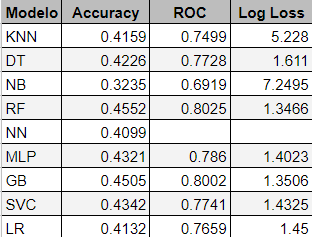
\includegraphics{models_metrics.png}
		\end{center}
		\caption{Resultados obetenidos por los algoritmos.\\ (\textbf{KNN}) K-Neirest Neighbors, 
		(\textbf{DT}) Decision Tree, (\textbf{NB}) Naive Bayes, (\textbf{RF}) Random Forest, (\textbf{NN}) Red neuronal implementada,
		(\textbf{MLP}) Multi-layer Perceptron, (\textbf{GB}) Gradient Boosting, (\textbf{SVC}) Support Vector Machine, (\textbf{LR}) Logistic Regression.  \label{results:fig}}%
	\end{figure}


	 
% %-----------------------------------------------------------------------------------
	 
%-----------------------------------------------------------------------------------
% 	\subsection{Listas y Descripciones}\label{sub:lists}
% %-----------------------------------------------------------------------------------
% 		Para producir listas enumeradas, use el siguiente estilo:

% %-----------------------------------------------------------------------------------
% 		\begin{enumerate}
% 			\item Primer Elemento
% 			\item Segundo Elemento
% 			%
% 			\begin {enumerate}
% 				\item {Segundo Elemento - Subitem Uno}
% 				\item {Segundo Elemento - Subitem Dos}
% 			\end {enumerate}
% 			%
% 		\end{enumerate}

% %-----------------------------------------------------------------------------------
% 		Para producir descripciones, use el siguiente estilo:

% %-----------------------------------------------------------------------------------
% 		\begin{description}
% 			\item [Primer Elemento] con su respectiva descripción.
% 			\item [Segundo Elemento] también con su respectiva descripción.
% 		\end{description}

%-----------------------------------------------------------------------------------
% 	\subsection{Figuras}\label{sub:figures}
% %-----------------------------------------------------------------------------------
% 		Para producir cuerpos flotantes (figuras ó tablas), asegúrese de numerar
% 		y etiquetar correctamente cada figura. Las referencias a las figuras deben
% 		estar también correctamente etiquetadas. Por ejemplo, en la Fig. \ref{fig:ex}
% 		se muestra\ldots.

% 		\begin{figure}[htb]%
% 		\begin{center}
% 			\emph{Aquí va el contenido de la figura \ldots}
% 		\end{center}
% 		\caption{Figura de ejemplo \label{fig:ex}}%
% 		\end{figure}

%-----------------------------------------------------------------------------------
% 	\subsection{Código Fuente}\label{sub:listings}
% %-----------------------------------------------------------------------------------
% 		Para producir código fuente, envuélvalo en una figura flotante y
% 		etiquételo correctamente. Por ejemplo, en la Fig. \ref{fig:code}
% 		se muestra un código bastante conocido\ldots.

% 		% Configuración de Listings
% 		\lstset{keywordstyle=\color{blue}, basicstyle=\small}

% 		\begin{figure}[htb]%
% 			\begin{lstlisting}[language=c]%

%     int main(int argc, char** argv)
%     {
%         // Imprimiendo "Hola Mundo".
%         printf("Hello, World");
%     }

% 			\end{lstlisting}
% 		\caption{Código fuente de ejemplo.\label{fig:code}}
% 		\end{figure}

%-----------------------------------------------------------------------------------
	% \subsection{Referencias}
%-----------------------------------------------------------------------------------
  	% Las referencias deben estar agrupadas en una sección al final del artículo,
  	% y las citas numeradas correctamente, por ejemplo \cite{knuth} ó \cite{goedel}.

  	% Incluya toda la información importante de cada referencia, incluídos autor,
  	% título, y notas de la edición. En caso de citar sitios web, además
  	% de la URL, incluya la fecha en que fue consultado, como en \cite{wiki}.

%===================================================================================



%===================================================================================
% Conclusiones
%-----------------------------------------------------------------------------------
\section{Conclusiones}\label{sec:conc}
	En este trabajo se ha definido el problema de selecci\'on de configuraciones 
	gr\'aficas como un problema de clasificaci\'on bajo el paradigma de
	aprendizaje supervisado y se ha realizado una comparaci\'on
	de distintos modelos presentes en la literatura para la realizaci\'on del mismo.
	Los resultados obtenidos fueron malos en todas las medidas utilizadas para su 
	evaluaci\'on sin embargo, esto nos ha permitido identificar causas potenciales que
	pueden llevar al pobre rendimiento de un sistema de recomendaci\'on de visualizaciones.

%   En esta sección puede incluir las conclusiones de su investigación y las ideas
%   sobre la continuidad del trabajo, en el caso que aplique.

%===================================================================================



%===================================================================================
% Recomendaciones
%-----------------------------------------------------------------------------------
\section{Recomendaciones y trabajo futuro}\label{sec:rec}

Se propone incorporar \textit{features} de pares de columnas y \textit{features} relacionados
con el \textit{dataset} y probar representaciones alternativas para modelar
este tipo de relaciones entre columnas como un grafo de conocimientos sobre el cual se puedan aplicar
algoritmos de clasificaci\'on de nodos. Adem\'as se propone incorporar nuevos modelos de redes neuronales
y optimizaci\'on de hiperpar\'ametros para estos modelos. Probar estos modelos en un corpus de dominio espec\'ifico
para determinar si la heterogeneidad de dominios es relevante en el resultado de los modelos.
%   En esta sección puede incluir recomendaciones sobre posibles formas de continuar
%   la investigación u otros temas relacionados.

%===================================================================================



%===================================================================================
% Bibliografía
%-----------------------------------------------------------------------------------
% \begin{thebibliography}{99}
%-----------------------------------------------------------------------------------
	
\bibliography{biblio}
% \bibitem{knuth} Donald E. Knuth. \emph{The Art of Computer Programming}.
	% 	Volume 1: Fundamental Algorithms (3rd~edition), 1997.
	% 	Addison-Wesley Professional.

	% \bibitem{goedel} Kurt Göedel. \emph{Über formal unentscheidbare Sätze der
	% 	Principia Mathematica und verwandter Systeme, I}.
	% 	Monatshefte für Mathematik und Physik 38.

	% \bibitem{wiki} Wikipedia. URL: \href{http://en.wikipedia.org}
	%   {http://en.wikipedia.org}.
	% 	Consultado en \today.

%-----------------------------------------------------------------------------------
% \end{thebibliography}

%-----------------------------------------------------------------------------------

\label{end}

\end{document}

%===================================================================================
